\chapter{\textbf{Contexto tecnológico de las antenas microstrip}}\label{ch:contexto}

En este capítulo veremos las características principales de las antenas microstrip. No entraremos en detalle con estudio analítico ya que no es objeto de este proyecto. Desde la sección~\ref{sec:conceptos} a la sección~\ref{sec:alimentacion} veremos los conceptos generales de análisis de las antenas microstrip. Prosiguiendo esta línea, en la sección~\ref{sec:aplicaciones} abordaremos las distintas aplicaciones de estas antenas y en la sección~\ref{sec:aplicacionesdmi} proporcionaremos una revisión bibliográfica de antenas microstrip para DMI.


\section{Conceptos básicos}\label{sec:conceptos}

Los elementos radiantes con característica microstrip fueron descritos originariamente por Deschamps en 1953~\cite{deschamps}. No fue hasta veinte años después, cuando se fabricaron las primeras antenas microstrip. El desarrollo durante la década de los setenta de mejores substratos y modelos teóricos más fiables, propició un crecimiento muy grande en el desarrollo de dichas antenas. A partir de la creación de la primera antena microstrip práctica por Howell y Munson~\cite{howell,munson}, se hicieron investigaciones exhaustivas sobre este campo y el uso de configuración en arrays de las mismas antenas~\cite{bahl,james1,james2}. Fueron muchas las ventajas descritas en ese momento respecto a otra clase de antenas, como por ejemplo su bajo peso y volumen, su reducido coste y además la facilidad de fabricarlas y depués configurarlas. Esto propició que se desarrollara en masa este tipo de antenas para diversos campos de estudio y aplicaciones, las cuales podremos ver en este capítulo.

Una \textbf{antena microstrip} consiste en un \textbf{parche} o \textbf{estructura radiante} formado de material conductor, que suele ser cobre, oro, aluminio, etc., colocado encima de una capa de \textbf{substrato dieléctrico} con una cierta permitividad relativa $\epsilon_{r}$ y por debajo de estas dos capas, \textbf{un plano de masa} de material conductor. Dicha antena puede ser alimentada de muchas maneras, a través de líneas microstrip, coaxiales u otros elementos radiantes, tal y como veremos en una próxima sección. Los materiales dieléctricos del substrato suelen tener una $\epsilon_{r}$ menor de 10 para no perder eficiencia en la antena~\cite{garg}.

\begin{figure}[!htb]
    \centering
    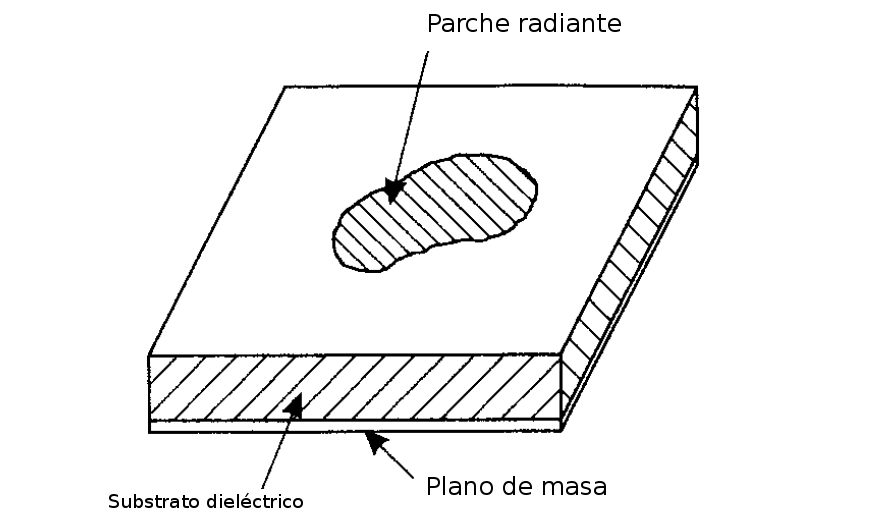
\includegraphics[scale=0.25]{./ContextoTecnologico/antena_parche}
    \caption{Dibujo de un esquema sencillo de una antena de parche o antena microstrip.}
    \label{fig:fig2.1}
\end{figure}

El conductor del parche como hemos dicho suele ser de un metal conductor con diversas formas geométricas posibles dependiendo de la aplicación y/o polarización requerida, aunque las más habituales suelen ser formas regulares (cuadrado, rectángulo, círculo, etc.). Para conseguir los campos que van hacia el exterior de la antena y ayudan a que aparezca la radiación, la constante dieléctrica  $\epsilon_{r}$ del substrato de la antena idealmente debe tener un valor bajo. Debido a esto, se han desarrollado varios tipos de substratos con óptimas propiedades en dicha variable, además de conseguir valores mínimos en pérdidas tangenciales\footnote{Término matemático que indica si es mayor la corriente de conducción o la corriente de desplazamiento cuando un campo electromagnético se propaga a través de cierto material. Proporciona las pérdidas de energía del dieléctrico.} del mismo dieléctrico. Estos materiales suelen ser moldeables, por lo que son apropiados para este tipo de antenas. Con respecto a los tipos de materiales utilizados para el substrato de una antena, éstos pueden ser de muchos tipos, entre los que destacamos: panal de miel (\textit{honeycomb}), cuarzo, grasas industriales, Duroid, ARLON1000, Macor, etc.

\clearpage

Muchas son las ventajas de las antenas de parche o microstrip, entre las que podemos enumerar~\cite{garg}:
\begin{itemize}
    \item Cubren aplicaciones que trabajan en un rango de frecuencias de 100 MHz a 100 GHz;
    \item Bajo peso, bajo volumen y configuraciones simples que pueden ser rediseñadas;
    \item Con una única alimentación, es posible obtener polarizaciones lineales y circulares;
    \item Su fabricación es muy simple y de bajo coste;
    \item Es posible crear antenas que trabajan en bandas duales;
    \item Pueden ser integradas perfectamente junto a circuitos de microondas;
    \item Algunas líneas y redes de alimentación pueden ser fabricadas simultáneamente junto a la estructura de la antena.
\end{itemize}

\begin{flushleft}
    Algunas de las limitaciones de las antenas microstrip son:
\end{flushleft}
\begin{itemize}
    \item Ancho de banda estrecho;
    \item Baja ganancia, alrededor de 6 dB;
    \item Es difícil conseguir una polarización pura;
    \item Un uso de un substrato de alta constante dieléctrica lleva asociado una pobre eficiencia y un reducido ancho de banda.
    \item Existe un constante compromiso entre muchas variables de la antena a fabricar: constante dieléctrica, ancho y largo, ancho del substrato, alimentación, etc.
\end{itemize}

Estas limitaciones pueden ser subsanadas si se aplican por ejemplo técnicas avanzadas que se alejan de nuestro estudio, como el uso de configuración array si se tiene una antena con muy baja ganancia~\cite{garg9}.


\section{Mecanismo de radiación}\label{sec:mecanismo}

La radiación de las antenas microstrip puede ser descrita en términos de distribución de campos alrededor de la superficie del parche conductor o de corrientes en la antena. Para calcular dicha distribución de campos de manera analítica hacen falta cálculos y métodos muy complejos~\cite{balanis14}, cosa que se aleja de nuestro estudio.

Para explicar el mecanismo de radiación, vamos a analizar de manera cualitativa una estructura muy sencilla de antena microstrip a la que se ha conectado una fuente de microondas. Como vemos en \textit{fig. \ref{fig:fig2.2}}, cuando el parche conductor recoge la energía procedente de la fuente, se establecen cargas entre la parte de arriba y la de abajo del propio parche conductor. Simultáneamente en el plano de masa se genera otra distrubución de cargas.

\begin{figure}[!htb]
    \centering
    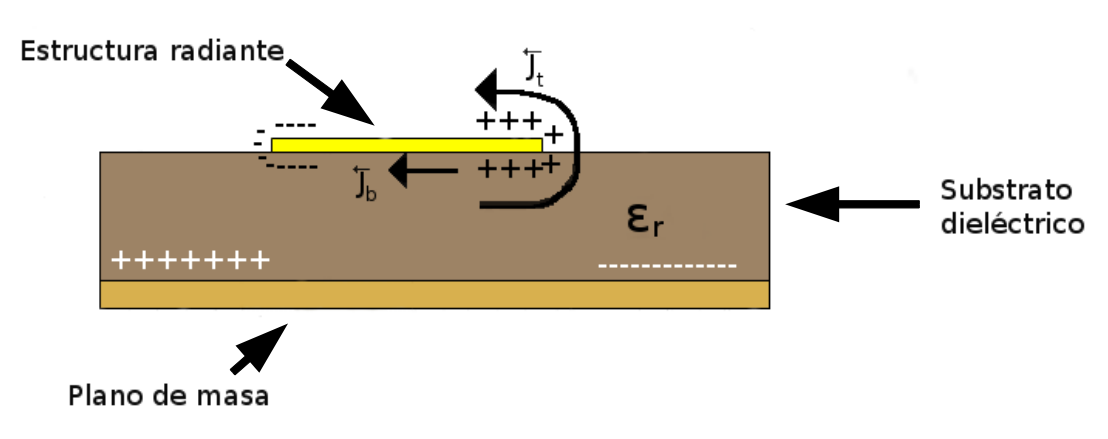
\includegraphics[scale=0.4]{./ContextoTecnologico/cargas_parche_4}
    \caption{Dibujo de las cargas de corriente que aparecen en la antena microstrip cuando se alimenta.}
    \label{fig:fig2.2}
\end{figure}

Las fuerzas resultantes repulsivas que aparecen entre las cargas de la parte de abajo del parche y la parte de la superficie, provocan un movimiento que desplaza a las cargas de abajo hacia arriba. Este movimiento crea dos \textbf{densidades de corriente} $\vec{J}$ tanto en la superficie como en la parte de abajo del parche. Es así como la fuerza atractiva entre las cargas predomina y debajo del parche es donde se acumula la mayor concentración de carga. Esto provoca pequeños flujos de corriente en los límites del parche hacia la superficie, siendo responsables de un débil campo magnético tangencial. Estas cargas además son el origen de los campos radiantes y de la radiación deseada, la cual puede ser aumentada utilizando un grosor mayor de substrato junto a un valor de $\epsilon_{r}$ suficientemente bajo para lograrlo. Sin embargo, la radiación de una estructura microstrip, tanto una antena como una línea, puede ser reducida si se utiliza un substrato dieléctrico con una alta constante relativa $\epsilon_r$ o en cambio, con una capa de substrato muy delgada. Por ello, las capas de substrato utilizadas deben ser anchas para permitir una radiación efectiva sin empeorar la eficiencia de dicha estructura. Como se puede deducir, existe un compromiso de diseño entre el ancho de la capa de substrato y el índice dieléctrico del material de la misma.


\section{Tipos de onda}\label{sec:ondas}

Tras ver cómo es posible el mecanismo de radiación, veremos qué tipos de ondas se forman en este tipo de antenas. Existen cuatro tipos de onda en una línea microstrip: las ondas espaciales, las ondas superficiales, las ondas de fuga y las ondas de guía \cite{balanis2}\cite{bhartia}.

\subsection{Ondas espaciales}\label{subsec:ondas-espaciales}

Las ondas espaciales son las ondas enviadas al espacio libre y sufren atenuación a medida que se alejan de su fuente. En el diseño de antenas, son las ondas más importantes a tener en cuenta, porque son las ondas radiadas. En el caso en el que se diseñan líneas de transmisión o circuitos, estas ondas son la causa de pérdidas y mal funcionamiento en la aplicación buscada y por tanto, deben eliminarse.

\subsection{Ondas superficiales}\label{subsec:ondas-superficiales}

Las ondas superficiales son las ondas que en su mayoría están recluídas dentro del substrato dieléctrico. No son ondas uniformes, ya que cuando viajan por esta capa son reflejadas una y otra vez por el plano de tierra y por la cara anterior del parche conductor. Las ondas superficiales permanecen viajando y perdiendo amplitud, tomando parte de la señal que se quiere enviar y aumentando las pérdidas en la transmisión. Esto provoca también un acoplamiento incorrecto del circuito de la antena.

\subsection{Ondas de fuga}\label{subsec:ondas-de-fuga}

Las ondas de fuga se forman cuando las ondas que viajan por el substrato dieléctrico llegan al lateral del substrato y se dividen entre las que se \textit{fugan} al espacio libre y las que se reflejan de nuevo.

\subsection{Ondas guiadas}\label{subsec:ondas-guiadas}

Las ondas guiadas aparecen en las antenas que tienen cubierto su parte superior casi por completo de material conductor: las ondas viajan por el substrato dieléctrico y al estar rebotando todo el rato por las partes metálicas, quedan recluídas dentro de la antena como si fuera un circuito. En el diseño de antenas esto se debe evitar.


\section{Alimentación}\label{sec:alimentacion}

Otro de los aspectos importantes del diseño de antenas, ya sean microstrip o de otro tipo, es el modelo de alimentación que tienen. Una antena con un mal diseño de alimentación puede llevar a un mal funcionamiento de la misma. A través de un correcto acoplamiento de impedancias, se puede conseguir que la antena radie en la banda de frecuencias deseada. Estudiaremos en nuestro caso tres métodos distintos: \textit{alimentación directa}, \textit{alimentación por proximidad} y \textit{alimentación por apertura} \cite{garg,bhartia}.

\subsection{Alimentación directa}\label{subsec:alimentacion-directa}

Este método de alimentación necesita que tanto la estructura de alimentación como el parche radiante estén unidos o en contacto. La principal desventaja de este método es que a la hora de diseñar, existe un compromiso muy estrecho entre las características de radiación de la antena y las características propias del modelo de alimentación. Ambas no se pueden optimizar por separado al estar unidas, ya que ambos se encuentran en una misma capa de substrato en la mayoría de diseños. Dentro de esta misma categoría de alimentación nos encontramos con dos tipos diferentes: la \textit{alimentación por microstrip} y la \textit{alimentación por coaxial}.

\subsubsection{Alimentación por microstrip}

La alimentación por microstrip o por tira conductora, consiste simplemente en alimentar al parche radiante por medio de una línea o tira microstrip con una impedancia diseñada con anterioridad. Este modelo es muy fácil de diseñar y fabricar pero conlleva no obstante una pérdida notoria en ancho de banda, acoplamiento y eficiencia. Las dos formas más comunes de alimentar una antena por medio de una tira microstrip son conectando la línea microstrip \textit{directamente en un borde de la antena} o alimentando la linea microstrip \textit{a través de inserciones en la antena}. El acoplamiento de impedancia dependerá de la posición de la línea con el parche radiante en el primer caso y en el segundo dependerá de la longitud de la inserción. Este método se aprecia en la \textit{fig. \ref{fig:fig2.3}}

\begin{figure}[!htb]
    \centering
    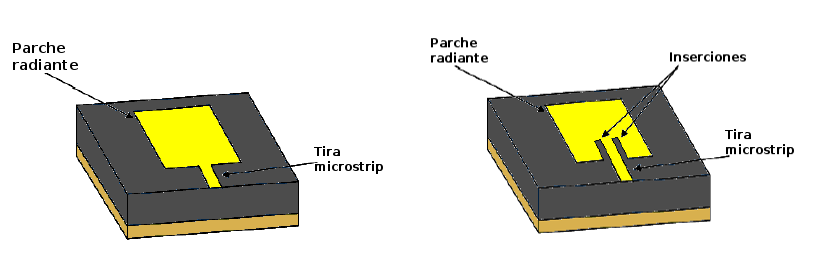
\includegraphics[scale=0.55]{./ContextoTecnologico/microstrip_feed}
    \caption{Ejemplo de antenas con alimentación microstrip. Izquierda: conexión directa al borde de la antena. Derecha: conexión con inserciones.}
    \label{fig:fig2.3}
\end{figure}

\subsubsection{Alimentación por coaxial}

La alimentación por coaxial se basa en colocar el pin del cable coaxial directamente al parche radiante y la parte negativa del pin a la capa de tierra o masa de la antena. Tendremos una impedancia u otra dependiendo de cómo coloquemos el coaxial con respecto a la antena y al parche radiante. Este método es uno de los más utilizados, pero su construcción es difícil ya que el pin del cable debe atravesar el substrato y a la vez estar soldado a la propia antena para su correcto funcionamiento. En la \textit{fig. \ref{fig:fig2.4}} podemos ver una estructura ejemplo.

\begin{figure}[!htb]
    \centering
    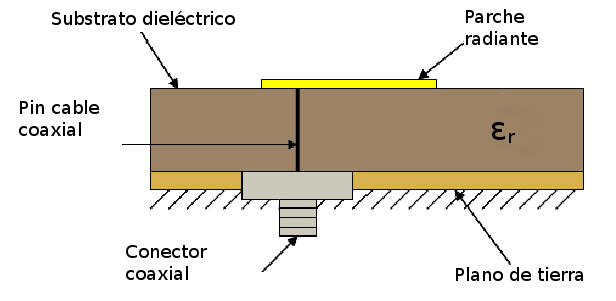
\includegraphics[scale=0.55]{./ContextoTecnologico/coaxial}
    \caption{Estructura ejemplo de una conexión para la alimentación por medio de un cable coaxial.}
    \label{fig:fig2.4}
\end{figure}

\subsection{Alimentación por proximidad}\label{subsec:alimentacion-por-proximidad}

La alimentación por proximidad ocurre en este caso por medio de un acoplamiento electromagnético. Consiste en separar la estructura del parche radiante de la estructura de alimentación para optimizar por separdo cada parte. Lo más normal es colocar el parche radiante en un substrato con una constante de permitividad relativa baja; debajo de éste la tira microstrip con un substrato con permitividad relativa alta y debajo de todas estas capas, el plano de masa o tierra. La \textit{fig. \ref{fig:fig2.5}} representa un ejemplo de la estrucutra de alimentación por proximidad.

\begin{figure}[!htb]
    \centering
    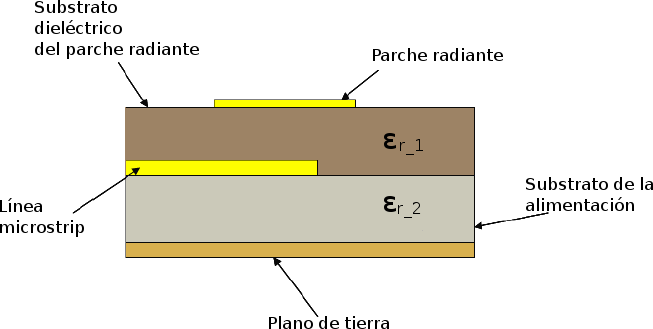
\includegraphics[scale=0.45]{./ContextoTecnologico/proximidad_2}
    \caption{Estructura ejemplo de la alimentación por proximidad.}
    \label{fig:fig2.5}
\end{figure}

\subsection{Alimentación por apertura}\label{subsec:alimentacion-por-apertura}

El método de alimentación por apertura consiste en diseñar una antena con estas capas: un parche radiante sobre un substrato dieléctrico, los cuales están encima de un plano de tierra compartido por otro substrato dieléctrico que tiene por debajo una línea microstrip de alimentación. Tiene muchas similitudes con el método de alimentación por proximidad, pero en este caso, el plano de tierra, que es común, tiene una apertura o agujero cuya posición y dimensiones participan directamente en el valor de la impendancia y por lo tanto, en el acoplamiento de la antena. Una ventaja a destacar con respecto a la alimentación por proximidad es que al estar más separadas las estructuras radiante y la de alimentación, la radiación de esta última no influye en la dirección de propagación de la onda resultante; evita además la aparición de interferencias y polarizaciones. Una estructura ejemplo se puede apreciar en la \textit{fig. \ref{fig:fig2.6}}.

\begin{figure}[!htb]
    \centering
    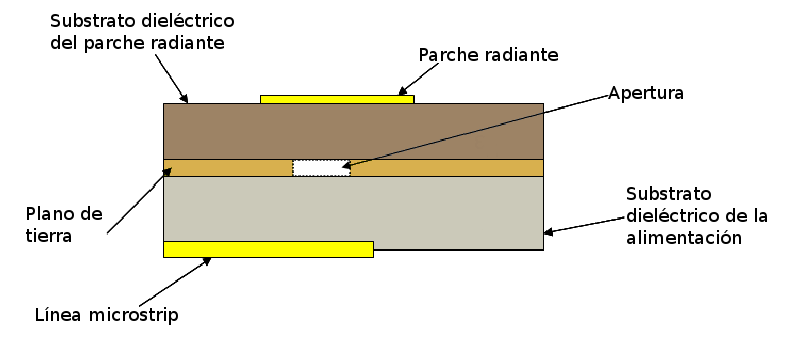
\includegraphics[scale=0.45]{./ContextoTecnologico/apertura}
    \caption{Estructura ejemplo de la alimentación por apertura.}
    \label{fig:fig2.6}
\end{figure}


\section{Antenas microstrip rectangulares}\label{rectangular}

Las antenas tipo parche rectangulares son las más utilizadas debido a su facilidad de diseño y de implementación en diversos dispositivos. Además de conseguir fácilemente la polarización, su estudio y análisis son bastante simples.

La configuración más sencilla posible de una antena microstrip es una antena en forma rectangular, cuyo parche conductor tiene dimensiones \textit{L} x \textit{W} (largo x ancho) situado encima de una capa de substrato con constante dieléctrica $\epsilon_r$ y anchura \textit{h}, la cual descansa sobre una última capa de plano de masa. Podemos ver esta estructura de antena en la \textit{fig. \ref{fig:fig2.7}}.

\begin{figure}[!htb]
    \centering
    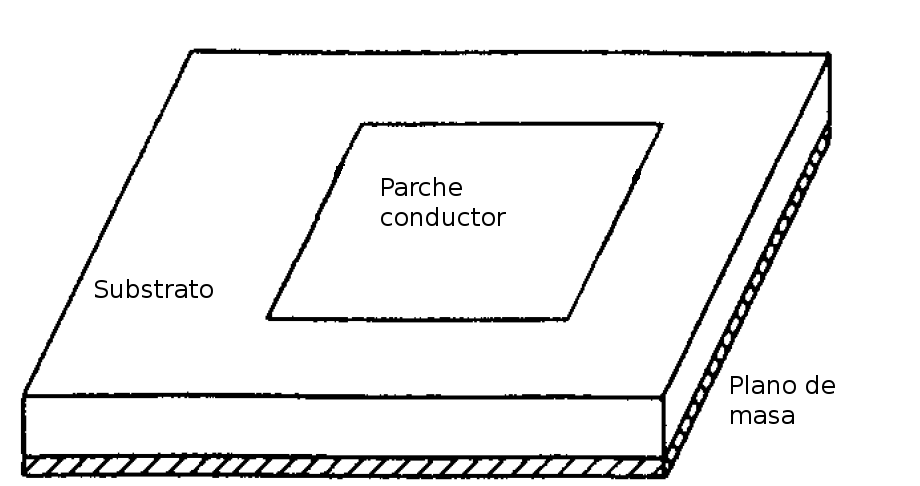
\includegraphics[scale=0.25]{./ContextoTecnologico/antena_rectangular}
    \caption{Dibujo ejemplo de una antena microstrip rectangular.}
    \label{fig:fig2.7}
\end{figure}

\subsection{Consideraciones de diseño}\label{subsec:consideraciones-de-diseno}

El objetivo principal del diseño es conseguir por ejemplo, un resultado específico a una frecuencia estipulada. En el diseño de una antena microstrip, el primer paso es la elección del tipo de substrato con una adecuada constante dieléctrica y el grosor de su capa $h$. Una capa ancha incrementa la potencia radiada, reduce las pérdidas por conducción e incrementa el ancho de banda. Sin embargo, esto aumenta el peso, las pérdidas del dieléctrico en sí y las pérdidas por ondas superficiales, además de las pérdidas por conectores. Es posible que una antena microstrip rectangular deje de emitir en su frecuencia de resonancia debido al grosor de esta capa y a la reactancia surgida en la alimentación~\cite{pozar}.\\

El valor de la constante dieléctrica $\epsilon_{r}$ es fundamental también para el diseño ya que un valor pequeño de éste incrementa el campo exterior radiado, la potencia radiada y por tanto la eficiencia de la antena; en cambio, un valor grande provoca todo lo contrario. Estudios realizados en \cite{garg4}, aseguran que el objetivo en el diseño es encontrar un substrato con índices de $\epsilon_{r}$ menores a 2,5.

Existe además un compromiso entre el grosor de la capa de substrato y la constante dieléctrica del mismo, ya que aumentar el ancho de la capa tiene el mismo efecto que disminuir $\epsilon_{r}$. Los elementos más utilizados para el substrato de antenas tipo parche son:

\begin{itemize}
    \item Honeycomb, con $\epsilon_{r}$ = 1.07;
    \item Duroid, con $\epsilon_{r}$ = 2.32;
    \item Cuarzo, con $\epsilon_{r}$ = 3.8;
    \item Arlon, con $\epsilon_{r}$ variable;
    \item y Alumina, con $\epsilon_{r}$ = 10.
\end{itemize}

Otras consideraciones parten del ancho $W$ y largo $L$ de la estructura de la antena. En~\cite{garg4} se sugiere que las dimensiones deben cumplir esta relación: $1 < W/L <2$. El ancho por ejemplo, afecta a la resistencia de entrada y al ancho de banda. El largo por otro lado, determina la frecuencia de resonancia y es crítico en el diseño debido a como hemos mencionado antes, el estrecho ancho de banda que proporcionan estas antenas. Puede incluso incrementar la potencia radiada, el ancho de banda y la eficiencia de radiación. No todos los campos quedan confinados en la región de $L$ x $W$ como se ha podido ver en en la sección~\ref{sec:ondas}; esto es lo que provoca realmente que la antena radie ondas electromagnéticas~\cite{garg4}.

\subsection{Métodos para el estudio de antenas microstrip rectangulares}\label{subsec:teoria}

En esta sección veremos dos modelos para el estudio de las antenas microstrip rectangulares los cuales facilitan mucho el estudio teórico y la asimilación de conceptos: el método de línea de transmisión y el método de cavidad.

\subsubsection{Método de línea de transmisión}

Las antenas microstrip tienen una estructura que deriva directamente de una línea de transmisión microstrip. En este modelo, la antena es modelada como una línea de transmisión de longitud L, una impedancia característica $Z_{0}$ y una constante de propagación que se deriva de la ecuación $\gamma = \alpha + j\beta$, donde $\alpha$ es la constante de atenuación de la línea y $\beta$ es la constante de fase de la misma. Los campos electromagnéticos varían a lo largo del parche, que suelen ser de media onda y la radiación se produce en este caso debido a los terminales que están en circuito abierto.\\

\begin{figure}[!htb]
    \centering
    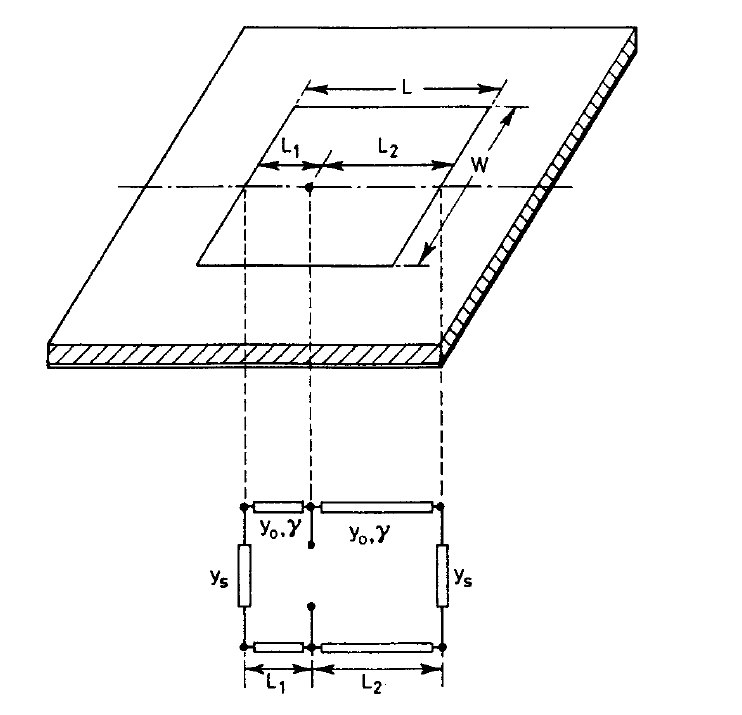
\includegraphics[scale=0.25]{./ContextoTecnologico/ejemplo_linea}
    \caption{Ejemplo de análisis de una estructura microstrip como línea de transmisión.}
    \label{fig:fig2.8}
\end{figure}

Existen muchos estudios sobre este método y la manera de desarrollar las ecuaciones del mismo para encontrar los parámetros de la línea, es decir cómo obtener la impendacia de entrada $Z_{in}$, la constante de fase $\beta$ y la auto-admitancia $Y_{S}$ (encontrada al final de la línea en circuito abierto y que recoge el efecto de la radiación de la línea)~\cite{munson,derneryd,pues}.

\subsubsection{Método de cavidad}

Otro punto de vista por el que podemos ver las antenas microstrip, es el de cavidad resonante. Las antenas microstrip son resonantes de banda estrecha, de ahí este nombre para este método de análisis.

En este modelo, el interior de la estructura de la antena es modelado como una cavidad rodeada de paredes eléctricas tanto en la parte inferior como superior y de una pared magnética a los lados. Existen unas bases para este modelo, asumiendo siempre que $h << \lambda_{0}$, es decir, que la altura de la capa de substrato sea mínima frente a la longitud de onda de resonancia \cite{richards}:

\begin{itemize}
    \item Los campos en el interior no varían con $z$, porque el substrato es muy delgado;
    \item El campo eléctrico viaja sólo en dirección $z$ y el campo magnético confinado entre el parche conductor y el plano de masa sólo tiene componentes $H_{x}$ y $H_{y}$;
    \item La corriente eléctrica en la dirección normal del parche conductor es cero, lo que implica que la componente tangencial del campo magnético a lo largo de los lados parche es cero y de esta forma la pared magnética está situada allí.
\end{itemize}

\begin{figure}[!htb]
    \centering
    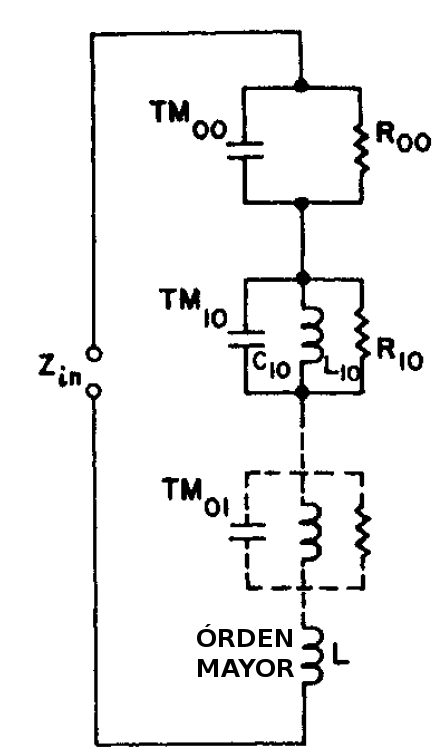
\includegraphics[scale=0.25]{./ContextoTecnologico/ejemplo_cavidad}
    \caption{Circuitos ejemplo tras el análisis del modelo de cavidad.}
    \label{fig:fig2.9}
\end{figure}

La distribución de campo está divida en dos regiones, los campos en el interior de la estructura y los campos que están en el exterior. Los campos externos son los que salen hacia afuera de la cavidad y determinan las características de radiación del parche. Así mismo, los campos internos de la cavidad nos proporcionan información acerca de la impendancia de entrada de la antena y las corrientes responsables de dicha radiación. Estos campos se determinan a través de las cuatro ecuaciones fundamentales del electromagnetismo descritas por Maxwell y su desarrollo para obtener la ecuación de onda.

Todo ese desarrollo determina la ecuación para obtener el campo eléctrico en la dirección de propagación $E_{z}$, la impedancia de entrada y fundamentalmente, los modos de trabajo de la cavidad. Los modos más básicos pueden ser representados mediante sencillos circuitos RLC como vemos en la \textit{fig \ref{fig:fig2.9}} \cite{garg4}.


\section{Aplicaciones}\label{sec:aplicaciones}

Las antenas microstrip o de tipo parche fueron inicialmente desarrolladas y utilizadas en aplicaciones militares, tales como diseño de misiles y/o cohetes, en la aviación y en la mejora de los sistemas de satélites \cite{garg1}. En la actualidad estas antenas han visto aumentado su uso en muchas otras áreas, debido especialmente al reducido coste de su fabricación. Es más, en muchas aplicaciones, las antenas convencionales pueden ser sustituidas por antenas de parche o microstrip.

\begin{flushleft}
    Algunas aplicaciones que han podido desarrollar antenas microstrip son:
\end{flushleft}

\begin{itemize}
    \item Comunicaciones vía satélite tipo broadcast (DBS);
    \item Radares Doppler y otros;
    \item Misiles y telemetría espacial;
    \item Alimentación en antenas con estructuras complejas;
    \item Comunicaciones móviles;
    \item Antenas integradas en dispositivos de comunicaciones;
    \item Elementos radiantes biomedicinales;
    \item Alarmas de intrusión.
\end{itemize}

Veremos a continuación con detalle algunas de estas interesantes aplicaciones en los campos de la comunicación terrestre y satélite, además de implementaciones para uso médico.

\subsection{Aplicaciones en comunicaciones móviles y vía satélite}\label{subsec:aplicaciones-en-comunicaciones-moviles-y-via-satelite}

Las comunicaciones móviles requieren dispositivos ligeros, pequeños y en consecuencia, antenas de bajo coste y poco volumen para integrar muchas otras herramientas \cite{james2}\cite{huang}. Las antenas microstrip cumplen este último propósito y para ello, se han desarrollado varios modelos de las mismas para distintas aplicaciones y sistemas de comunicaciones móviles. Muchas de estas antenas que trabajan en rangos que van de MHz a GHz han sido integradas en radares, barcos, aviones, teléfonos celulares e incluso en sistemas automovilísticos para evitar colisiones.

Las antenas aplicadas a las comunicaciones vía satélite utilizan en algunas aplicaciones la polarización circular. Para ello, se diseñan antenas microstrip con forma de parche circular con uno o más puntos de alimentación en ella \cite{garg8}. Pero existen algunos problemas en el desarrollo de estas antenas, como por ejemplo el límite de potencia que puede dar el satélite o el tamaño máximo de la antena o incluso, la ganancia de la misma para obtener una fiable comunicación entre el satélite y la Tierra. Es en este caso cuando se han diseñando arrays de antenas microstrip, consiguiendo mucha más directividad, ganancia y bajo coste en la implementación. Muchas de ellas son construidas bajo el criterio de uso de unos modos de onda concretos TM.

Otra interesante aplicación vía satélite que empezó siendo un proyecto militar hace 30 años y ahora es una realidad cotidiana es el \textbf{GPS} o \textbf{Sistema de Posicionamiento Global} \cite{garg1}. Actualmente, este sistema es utilizado por millones de dispositivos o vehículos en cualquier parte del mundo para determinar su posición y altura de manera exacta. El GPS consiste en 24 satélites que orbitan alrededor de la Tierra a unos 20.000 kms. de distancia. Para obtener este servicio, se necesitan antenas de polarización circular omnidireccionales y de baja ganancia. Las antenas microstrip son adecuadas para este trabajo, minimizando el tamaño de la antena, el peso y el coste de la misma en la banda L de frecuencias (1573-1577 MHz), que es la que utiliza el GPS.

Las aplicaciones correspondientes a las comunicaciones móviles terrestres es el campo donde el desarrollo e integración de las antenas microstrip está extendido globalmente \cite{garg1}. Las antenas que normalmente llevan los dispositivos celulares suelen ser de pequeño tamaño y por supuesto compactas. Un problema existente en este tipo de comunicaciones es la baja eficiencia y ganancia de las antenas. El problema puede ser resuelto modificando el diseño de las antenas mediante substratos con un dieléctrico con $\epsilon_r$ más alto o incluso colocando arrays de antenas.

\subsection{Aplicaciones en medicina}\label{subsec:aplicaciones-en-medicina}

Las ondas de microondas han sido estudiadas profundamente en el campo de la medicina como una manera efectiva de combatir la hipotermia y tratar tumores malignos. Un elemento radiante que se utilice para estos propósitos y que se aplique directamente en la superficie a tratar debe ser ligero, flexible y fácil de manejar. Este elemento por ejemplo puede ser un parche con estructura radiante.

Algunos diseños de estructuras microstrip utilizadas son los dipolos impresos o los anillos anulares en la banda S para tratar la hipotermia \cite{sterzer}. Hay otros casos de discos circulares microstrip en la banda L para el mismo cometido \cite{deleo}. En otro caso, para medir la temperatura del cuerpo humano, se ha utlizado dos líneas microstrip con separación variable y ajustable~\cite{kobay1}. Un uso de esta aplicación, la cual va encaminada a nuestro estudio, se puede ver en la \textit{fig. \ref{fig:fig2.10}}.

\begin{figure}[!htb]
    \centering
    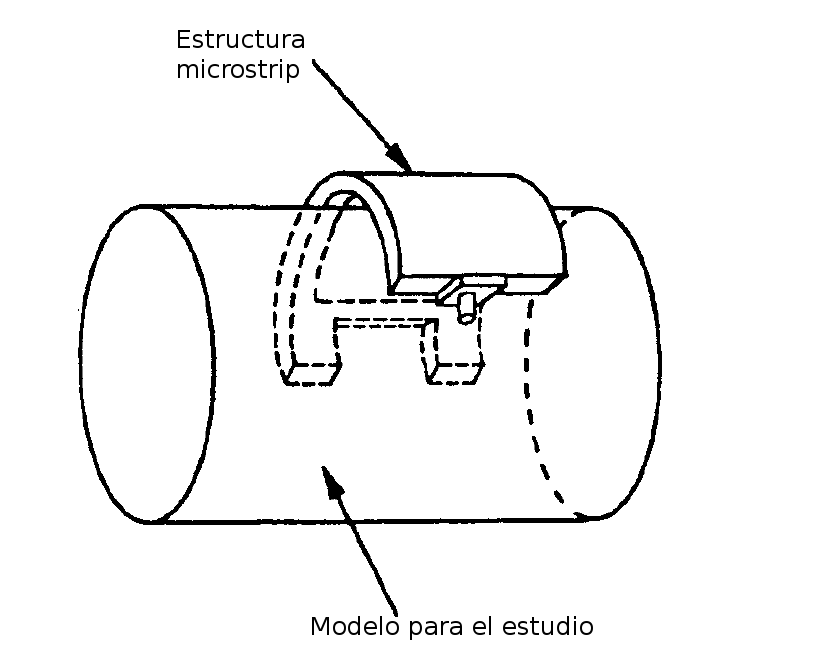
\includegraphics[scale=0.2]{./ContextoTecnologico/antena_medicina}
    \caption{Ejemplo de aplicación de una estructura microstrip flexible para uso medicinal trabajando a una frecuencia de 430 MHz. \cite{kobay2}}
    \label{fig:fig2.10}
\end{figure}


\section{Antenas microstrip en dispositivos médicos implantables}\label{sec:aplicacionesdmi}

En la anterior sección, se han mencionado algunas de las aplicaciones más destacables de las antenas microstrip, con especial mención de la última parte para uso médico. A lo largo de la actual sección, vamos a citar algunos ejemplos de diseños de antenas microstrip para sistemas de comunición de los DMI.

En la literatura acerca de diseños de antenas microstrip para DMI podemos encontrar múltiples estudios. En \textit{Antennas for Over-Body-Surface Communication at 2.45 GHz} de Conway et al. \cite{conway} tenemos un ejemplo de diseño de antenas microstrip para la comunicación de DMI colocados a lo largo de la superficie del cuerpo. En este caso los autores intentan máximizar el parámetro $S_{21}$ entre dos o más dispositivos para conseguir una enlace de comunicaciones fiable. Las antenas microstrip emiten a la frecuencia 2.45 GHz, centrados en la banda ISM (\textit{Industrial, Scientific and Medical band}), frecuencia en la que los autores estudian la posibilidad de tener ondas que se propagan a lo largo de la superficie del cuerpo. Para ello, en el artículo se proponen cinco tipos de antenas microstrip y se realiza un estudio paramétrico de cada una de ellas para la banda mencionada.

\begin{figure}[!htb]
    \centering
    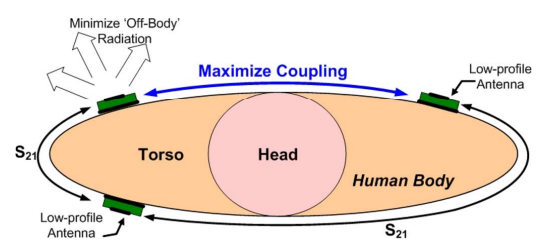
\includegraphics[scale=0.4]{./ContextoTecnologico/articulos/conway1}
    \caption{Esquema del estudio de antenas microstrip sobre la superficie del cuerpo para su comunicación obtenido del artículo \cite{conway}.}
    \label{fig:fig2.11}
\end{figure}

Tras algunas simulaciones y pruebas reales en laboratorio con las antenas, los autores concluyen que el tipo de antena HMMPA (\textit{Higher Mode Microstrip Patch Antenna}), es decir, antenas tipo parche con un alto modo de propagación de onda, son las más adecuadas para este tipo de investigación, ya que obtienen unos resultados parecidos a antenas tipo monopolo\footnote{Antenas formadas por un solo brazo rectilíneo en posición vertical.}. El parámetro $S_{21}$ que obtienen es eficiente y no hay tanta pérdida de potencia como en otras antenas.\\

Otro artículo interesante es el titulado \textit{Dual-band microstrip patch antenna based on short-circuited ring and spiral resonators for implantable medical devices}~\cite{requena} escrito por C.J. Sánchez-Fernández et al., en el cual se propone un diseño innovador para el parche radiante de las antenas microstrip. El parche está formado por una espiral y un anillo cortocircuitado, con lo que proporciona a la antena la característica de ser dual, es decir, que pueda emitir en dos bandas de frecuencias. Este esquema lo podemos ver en la \textit{fig. \ref{fig:fig2.12}}. En este caso, la antena es capaz de emitir tanto en la banda MICS (\textit{Medical Implant Communication Service band}) (402-405 MHz) como en la banda ISM (\textit{Industrial, Scientific and Medical band}) (2.4-2.48 GHz). El diseño de la antena está compuesto de dos capas de substrato dieléctrico: un superestrato para proteger al parche y un substrato para conseguir el efecto de radiación.

\begin{figure}[!htb]
    \centering
    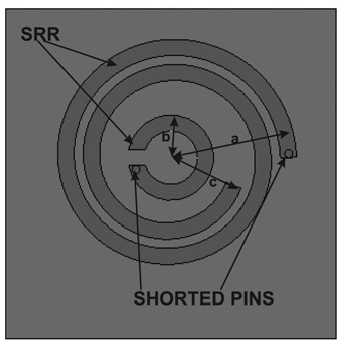
\includegraphics[scale=0.4]{./ContextoTecnologico/articulos/requena1}
    \caption{Diseño del parche radiante la antena microstrip dual descrita en \cite{requena}.}
    \label{fig:fig2.12}
\end{figure}

La espiral del parche hace que la antena radie en la banda MICS y el anillo cortocircuitado en la banda ISM. Los autores realizan diversos experimentos en simulación con la antena sobre distintos medios, como el entorno muscular, el entorno de tres tejidos (piel, músculo y grasa) y en un modelo de cuerpo humano completo. Una de las ventajas que posee esta antena es su reducido tamaño respecto a otras antenas microstrip para DMI. La alimentación de la antena, que es a partir del método de proximidad, consigue un nivel de libertad mayor respecto a otras antenas, sujetas a la alimentación por medio de conexiones coaxiales u otro tipo. Los autores concluyen argumentando que la antena cumple su misión presentando las pruebas realizadas en laboratorio del parámetro $S_{11}$ medidas en un gel con características parecidas al tejido humano de la piel.\\

Un nuevo diseño de antena microstrip lo podemos encontrar en el artículo llamado \textit{Implanted Antennas Inside a Human Body: Simulations, Designs, and Characterizations} \cite{kim}, escrito por J. Kim y Y. Rahmat-Samii. En el artículo, a parte de mencionar los distintos tipos de simulaciones y caracterizaciones que se pueden realizar de un estudio electromagnético para DMI, se propone un diseño de parche radiante en forma de serpentina. Es una antena de bajo coste, pequeña y eficiente que emite en la banda MICS.

\begin{figure}[!htb]
    \centering
    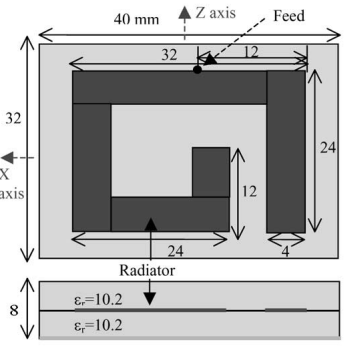
\includegraphics[scale=0.4]{./ContextoTecnologico/articulos/kim1}
    \caption{Diseño del parche radiante en forma de espiral de la antena microstrip descrita en \cite{kim}.}
    \label{fig:fig2.13}
\end{figure}

El diseño propuesto permite tener una antena mucho más peqeuña que otros diseños ya que la estructura en espiral, al igual que hemos visto en el ejemplo anterior, reduce el tamaño de la antena considerablemente. En cambio, se pierde eficiencia al no tener unas capas de substrato lo suficientemente anchas y grandes que permitan la radiación hacia el exterior.

A lo largo del artículo se hace un estudio sobre la comunicación entre la antena diseñada y otra externa tipo dipolo de media longitud de onda. La antena en espiral está situada en un torso humano diseñado en 3D, que podemos visualizar en la \textit{fig. \ref{fig:fig2.14}}.

Los resultados mostrados indican que el enlace de comunicaciones es posible de esta manera y que por supuesto cumplen con los límites legales de radiación máxima permitida para el cuerpo humano. Los autores concluyen argumentando que para este tipo de simulaciones en 3D del torso humano, es conveniente incluir parte del cuello y hombros, para obtener una correcta distribución de campos.

\vspace{1.5cm}

\begin{figure}[!htb]
    \centering
    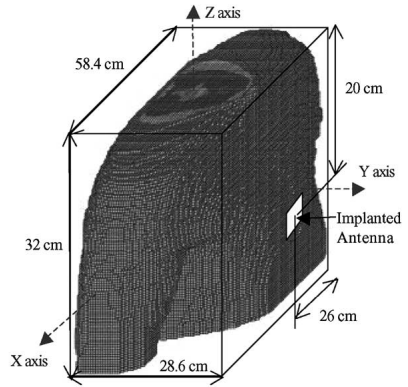
\includegraphics[scale=0.3]{./ContextoTecnologico/articulos/kim2}
    \caption{Diseño 3D del torso de cuerpo humano para simular la antena microstrip descrita en \cite{kim}.}
    \label{fig:fig2.14}
\end{figure}

Siguiendo la línea del anterior artículo, se diseña otra antena microstrip, pero esta vez con parche radiante en forma de serpentina en el artículo escrito por T. Karacolak et al. y titulado \textit{Design of a Dual-Band Implantable Antenna and Development of Skin Mimicking Gels for Continuous Glucose Monitoring}~\cite{karacola}. La gran diferencia con el anterior artículo se basa en que este nuevo diseño permite a la antena ser una antena dual, que trabaje tanto en la banda MICS, como en la banda ISM. Las dimensiones de la antena son reducidas de nuevo, obteniendo una antena apta para DMI.

\begin{figure}[!htb]
    \centering
    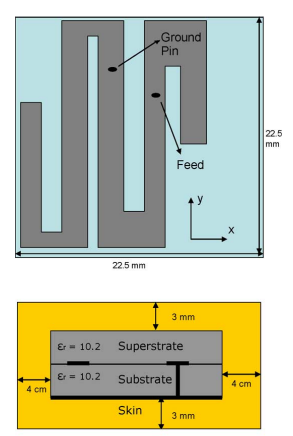
\includegraphics[scale=0.25]{./ContextoTecnologico/articulos/kara1}
    \caption{Diseño de la antena dual en forma de espiral descrita en \cite{karacola}.}
    \label{fig:fig2.15}
\end{figure}

\clearpage

La característica de la antena que le permite trabajar en las dos bandas es conseguida a través de diferencias en el parche radiante. En el anterior ejemplo~\cite{kim}, el ancho del parche era igual en toda su longitud, pero en este caso, se puede apreciar que hay distintos grosores a lo largo de la longitud. Sumando a esto, la antena posee un pin unido a tierra que hace cortocircuito para diferenciar cuándo empieza una banda y otra. En la \textit{fig. \ref{fig:fig2.16}} podemos apreciar estos detalles.

\begin{figure}[!htb]
    \centering
    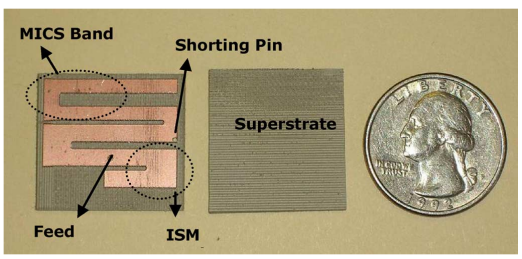
\includegraphics[scale=0.4]{./ContextoTecnologico/articulos/kara2}
    \caption{Antena dual fabricada basada en el diseño descrito en \cite{karacola}.}
    \label{fig:fig2.16}
\end{figure}

El artículo hace también un completo estudio sobre distintos geles que imitan a las propiedades el tejidos humanos para pruebas en la banda MICS. Los autores concluyen su artículo mostrando que la antena es eficiente en ambas bandas y cumplen su tarea a través de gráficas del parámetro $S_{11}$ y diagramas de radiación. Como línea futura, incluyen que están trabajando sobre un gel que funcione mejor para la banda ISM.
